\documentclass{report}
\usepackage{pdfpages}
\usepackage{graphicx} 
\usepackage{dirtytalk}
\usepackage{lmodern}
\usepackage{booktabs}
\usepackage{listings}
\usepackage{float}
\usepackage{siunitx}
\usepackage{amsmath}
\usepackage{rotating}
\usepackage{arydshln}
\usepackage[ngerman]{babel}
\usepackage[a4paper, total={6in, 8in}]{geometry}
\begin{document}

\includepdf[pages=-]{./PDFs/Deckblatt_P1}
\begin{titlepage}
    \begin{center}
        \vspace*{1cm}
            
        \Huge
        \textbf{Auswertung und Protokoll}
            
        \vspace{0.5cm}
        \LARGE
        Zum Versuch: MOS - Mechanischer Oszillator
        
        \vspace{1.8cm}

        \textbf{Jonas Müther \& Alejandro Schultheiss}
        \vfill
            
        P1 Praktikum\\
       
            
        \vspace{0.8cm}
  

        \vspace{1.8cm}
        \Large
        LMU München \\
        Physik B.Sc.\\
        Deutschland\\
        2026
            
    \end{center}
\end{titlepage}
\tableofcontents

\newpage
\chapter{Vorbereitung}

\section{Versuchsvorbereitung und Grundlagen des Versuchs}
\includepdf[pages=-]{./PDFs/VorbereitungMOS.pdf}

\section{Versuchsprotokoll}
\includepdf[pages=-]{./PDFs/MOS_Durchfuehrung.pdf}

\newpage
\chapter{Auswertung}
\section{Teilversuch I: Bestimmung der Erdbeschleunigung mithilfe eines Fadenpendels}
\subsection{Theoretischer Hintergrund}
In Teilversuch I wurde ein Fadenpendels frei schwingen gelassen. Aus der gemessenen Schwingungsdauer sollte dann die Erdbeschleunigung ermittelt werden.
Dies ist aufgrund folgender Herleitung für die Zusammenhang zwischen Erdbeschleunigung $g$ und der Schwingungsdauer $T$ möglich.
Hierzu betrachten wir Abbildung \ref{fig:KraefteFadenpendel}:
\begin{figure}[H]
    \centering
    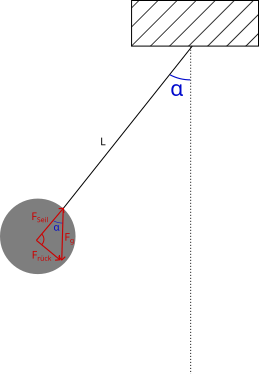
\includegraphics[width=0.4\textwidth]{./Images/Fadenpendel.png}
    \caption{Kräfte Fadenpendel}
    \label{fig:KraefteFadenpendel}
\end{figure}
Nach der Abbildung gilt für die Rücktreibende Kraft bei einem Auslenkungswinkel $\alpha$:
\begin{equation}
    \begin{split}
    F_{rueck}   &= F_g \cdot sin(\alpha) \\
                &= mg \cdot sin(\alpha)
    \end{split}
\end{equation}
Da im Bogenmaß $\alpha = \frac{s}{l}$ gilt, folgt:
\begin{equation}
    F_{rueck} = mg \cdot sin(\frac{s}{l})
\end{equation}
Für kleine Winkel gilt im Bogenmaß: $sin(x) \approx x$.
Somit gilt für kleine Winkel:
\begin{equation}
    F_{rueck} = mg \cdot \frac{s}{l}
\end{equation}
Diese Rücktreibende Kraft bewirkt eine Beschleunigung ($F = ma$), sodass folgt:
\begin{equation}
    \begin{split}
        ma + mg \frac{s}{l} &= 0\\
        \Leftrightarrow \ddot{s} + g \cdot \frac{s}{l} &= 0\\
        \Leftrightarrow \ddot{s} + \frac{g}{l} \cdot s &= 0
    \end{split}
\end{equation}
Um diese Differentialgleichung zu lösen verwendet man einen Exponentialansatz:
\begin{equation}
    s(t) = c \cdot e^{\lambda t}
\end{equation}
Die zweite Ableitung dieses Ansatzes ergibt:
\begin{equation}
    \ddot{s}(t) = {\lambda}^2 \cdot s(t)
\end{equation}
Setzt man den Ansatz in die Differentialgleichung ein, folgt:
\begin{equation}
    \begin{split}
    {\lambda}^2 \cdot s(t) + \frac{g}{l} \cdot s(t) = 0 \\
    \Leftrightarrow ({\lambda}^2 + \frac{g}{l}) \cdot s(t) = 0
    \end{split}
\end{equation}
Da diese Gleichung für alle Zeiten gelten muss, folgt:
\begin{equation}
    \begin{split}
        {\lambda}^2 &= -\frac{g}{l} \\
        \Leftrightarrow \lambda_{1,2} &= \pm i\sqrt{\frac{g}{l}} \\
        \Leftrightarrow \lambda_{1,2} &= \pm i \omega_0
    \end{split}
\end{equation}
Wobei $\omega_0 = \sqrt{\frac{g}{l}}$ die Eigenfrequenz der Schwingung ist.
Somit ergibt sich für die Lösung der Differentialgleichung:
\begin{equation}
    s(t) = c_1 e^{i \omega_0 t} + c_2 e^{-i \omega_0 t}
\end{equation}
wobei $c_1$ und $c_2$ durch die Anfangsbedingungen der Schwingung festgelegt sind.
Für den Zusammenhang zwischen Periodendauer $T$ und der Erdbeschleunigung $g$ der Schwingung gilt dann:
\begin{equation}
    \begin{split}
        T &= \frac{2 \pi}{\omega_0} \\
        \Leftrightarrow T &= 2 \pi \sqrt{\frac{l}{g}} \\
        \Leftrightarrow g &= 4 {\pi}^2 \frac{l}{T^2}
    \end{split}
    \label{eq:gAusT}
\end{equation}

\subsection{Auswertung der Messwerte}
Aus den bestimmten Dauern für 20 Schwingungen ergeben sich mit $T_i = \frac{t_i}{20}$ die in Tabelle \ref{tab:PeriodeMessdurchlaeufe}
\begin{table}[H]
    \centering
    \caption{Experimentelle Periodendauern der verschiedenen Messdurchläufe}
    \label{tab:PeriodeMessdurchlaeufe}
    \begin{tabular}{c | c}
        \hline
        Messdurchlauf & $T_i$ (s) \\
        \hline
        1 & 1.4465\\
        2 & 1.4475\\
        3 & 1.4415\\
        4 & 1.4510\\
        5 & 1.4440\\
    \end{tabular}
\end{table}
Der Mittelwert dieser Messwerte ist gegeben durch das Arithmetische Mittel:
\begin{equation}
    \begin{split}
        \bar{T} &= \frac{1}{n} \sum_{i=1}^{n} T_i \\
                &= \frac{1.4465s + 1.4475s + 1.4415s + 1.4510s + 1.4440s}{5} \\
                &= 1.4461s
    \end{split}
\end{equation}
Die Standardabweichung ($\sigma$) dieses Mittelwerts ergibt sich folgendermaßen:
\begin{equation}
    \begin{split}
        \sigma  &= \sqrt{\frac{1}{n-1}\sum_{i=1}^{n} (T_i - \bar{T})^2} \\
                &= (3.60 \cdot 10^{-3})s
    \end{split}
\end{equation}
Die Unsicherheit des Messwerts ergibt sich dann aus der Standardabweichung:
\begin{equation}
    \begin{split}
        \Delta T &= \frac{\sigma}{\sqrt{n}} \\
                 &= \frac{3.6 \cdot 10^{-3}s}{\sqrt{5}} \\
                 &\approx (1.7 \cdot 10^{-3})s
    \end{split}
\end{equation}
Somit gilt:
\begin{equation*}
    \boxed{T = (1.4461 \pm 0.0017)s}
\end{equation*}

Als Länge bis zum Schwerpunkt der Kugel wurde ein Wert von
\begin{equation*}
    l = (516.8 \pm 2.1)mm
\end{equation*}

Daraus ergibt sich mithilfe von Formel \ref{eq:gAusT} ein experimenteller Mittelwert für g.
\begin{equation}
    \begin{split}
        \bar{g} &= 4 {\pi}^2 \frac{516.8 \cdot 10^{-3}m}{(1.4451s)^2} \\
                &= 9.770m/s^2
    \end{split}
\end{equation}

Die Unsicherheit dieses Wertes errechnet sich mit folgender Formel:
\begin{equation}
    \begin{split}
        \Delta g &= \sqrt{(\frac{\partial g}{\partial T} \Delta T)^2+(\frac{\partial g}{\partial l} \Delta l)^2} \\
                 &= \sqrt{(-8 \pi^2 \frac{l}{T^3} \Delta T)^2 + (\frac{4 \pi^2}{T^2} \Delta l)^2} \\
                 &= \sqrt{(-8 \pi^2 \frac{0.5168m}{(1.4451s)^3} \cdot 0.0017s)^2 + (4 \pi^2 \frac{0.0021m}{(1.4451s)^2})^2} \\
                 &= 0.046 m/s^2 \\
                 &\approx 0.05 m/s^2
    \end{split}
\end{equation}

Als experimentell bestimmter Wert für die Erdbeschleunigung $g_{exp}$ ergibt sich also:
\begin{equation*}
    \boxed{g_{exp} = (9.77 \pm 0.05)m/s^2}
\end{equation*}

Es gilt:
\begin{equation}
    \begin{split}
        \bar{g}_{exp} + \Delta g  &= 9.82m/s^2 \\
                        > g_{lit} &= 9.8073m/s^2 \\
       > \bar{g}_{exp} + \Delta g &= 9.72m/s^2
    \end{split}
\end{equation}
Somit stimmt der experimentell bestimmte Wert von $g$ im Rahmen der Unsicherheit mit dem Liteaturwert überein.

\newpage
\section{Teilversuch II: }

\newpage
\section{Teilversuch II: }

\newpage
\section{Teilversuch III: }

\newpage
\section{Teilversuch IV: }

\newpage
\chapter{Anhang}
\section{SCRIPTS}

\definecolor{codegreen}{rgb}{0,0.6,0}
\definecolor{codegray}{rgb}{0.5,0.5,0.5}
\definecolor{codepurple}{rgb}{0.58,0,0.82}
\definecolor{backcolour}{rgb}{0.95,0.95,0.92}

\lstdefinestyle{matlab}{
    backgroundcolor=\color{backcolour},   
    commentstyle=\color{codegreen},
    keywordstyle=\color{magenta},
    numberstyle=\tiny\color{codegray},
    stringstyle=\color{codepurple},
    basicstyle=\ttfamily\footnotesize,
    breakatwhitespace=false,         
    breaklines=true,                 
    captionpos=b,                    
    keepspaces=true,                 
    numbers=left,                    
    numbersep=5pt,                  
    showspaces=false,                
    showstringspaces=false,
    showtabs=false,                  
    tabsize=2
}

\end{document}
